\documentclass[10pt,a4paper]{article}
\usepackage[utf8]{inputenc}
\usepackage[T1]{fontenc}
\usepackage{amsmath}
\usepackage{amsfonts}
\usepackage{amssymb}
\usepackage{graphicx}
\usepackage{tikz}
\usepackage{float}
\usepackage{tikz-cd}

\usepackage[backend = biber, style=authoryear]{biblatex}
\addbibresource{bibliography.bib}

\usetikzlibrary{fit,positioning}

\author{Gabriel Wallin}
\title{Some notes on state-space LBM}

\begin{document}
\maketitle

\section{SIR model}
To specify the State-Space Latent Block Model (SS-LBM), we introduce the following notation: 
%
$
\mathbf{y} = (\mathbf{y}_{ij}, i = 1, \ldots, n; j = 1, \ldots d) 
$
%
denotes the data matrix. Each element in $\mathbf{y}_{ij}$ is a multivariate time series:  
%
$
\mathbf{y}_{ij} = (y_{ij}^1(t), \ldots, y_{ij}^S(t))
$ 
%
where $t \in [0, T]$. In the context of analyzing the 2020 coronavirus pandemic, 
%
$
\mathbf{y}_{ij} = (y_{ij}^I(t), y_{ij}^R(t))^\top
$
%
where $y_{ij}^I(t)$ and $y_{ij}^R(t)$ denote the proportion of infected and removed (recovered or dead) by the virus, respectively, at time point $t$. Further, let  
%
$
\boldsymbol{\theta} = (\theta_t^S, \theta_t^I, \theta_t^R)^\top,
$
%
where $\theta_t^S$, $\theta_t^I$ and $\theta_t^R$ is the probability of a person being susceptible, infected and removed, respectively, at time point $t$. We will assume that 
%
$
\boldsymbol{\theta}_{0:T} = (\boldsymbol{\theta}_0, \boldsymbol{\theta}_1, \ldots, \boldsymbol{\theta}_T)
$
%
is a first-order Markov chain in the same spirit as \parencite{osthus2017forecasting} and \parencite{song2020epidemiological}. This implies that 
%
$
g(\boldsymbol{\theta}_t|\boldsymbol{\theta}_{0:(t-1)}) = g(\boldsymbol{\theta}_t|\boldsymbol{\theta}_{t-1}) \, \forall t \in [0:T]. 
$
%
Specifically, we assume the following model for $\boldsymbol{\theta}$:
%
$$
\boldsymbol{\theta}_t | \boldsymbol{\theta}_{t-1}, \boldsymbol{\tau} \sim \text{Dirichlet}(\kappa f(\theta_{t-1}^S), \kappa f(\theta_{t-1}^I), \kappa f(\theta_{t-1}^R)),
$$
where $\kappa$ scales the variance of the Dirichlet distribution, and the function $f(\cdot)$ is a 3-dimensional vector that sets the mean of the Dirichlet distribution.
%

The function $f$ is the solution to the following dynamic system:
%
\begin{equation}\label{SIR}
	\frac{\theta_t^S}{dt} = -\rho\theta_t^S\theta_t^I, \quad \frac{\theta_t^I}{dt} = \rho\theta_t^S\theta_t^I - \pi \theta_t^I, \quad \frac{\theta_t^R}{dt} = \pi \theta_t^I,
\end{equation}
%
where $\rho > 0$ is the transmission rate of the disease and $\pi > 0$ is the rate of recovery. This system of non-linear ordinary differential equations is within the field of epidemiology known as the SIR model \parencite{kermack1927contribution}. Since there are no explicit solutions available to (\ref{SIR}), the so-called fourth-order Runge-Kutta approximation is implemented, meaning that 
%
$$
\begin{aligned}
	\begin{pmatrix}
		f(\theta_{t-1}^S) \\
		f(\theta_{t-1}^I) \\
		f(\theta_{t-1}^R)
	\end{pmatrix}
\end{aligned} = 
%
\begin{aligned}
	\begin{pmatrix}
		\theta_{t-1}^S + 1/6[k_{t-1}^{\theta^S_1} + 2k_{t-1}^{\theta^S_2} + 2k_{t-1}^{\theta^S_3} + k_{t-1}^{\theta^S_4}] \\
		\theta_{t-1}^I + 1/6[k_{t-1}^{\theta^I_1} + 2k_{t-1}^{\theta^I_2} + 2k_{t-1}^{\theta^I_3} + k_{t-1}^{\theta^I_4}] \\
		\theta_{t-1}^R + 1/6[k_{t-1}^{\theta^R_1} + 2k_{t-1}^{\theta^R_2} + 2k_{t-1}^{\theta^R_3} + k_{t-1}^{\theta^R_4}]
	\end{pmatrix}
\end{aligned}
$$
%
where 
%
\begin{equation*}
\begin{split}	
		k_{t-1}^{\theta^S_1} &= - \rho \theta_{t-1}^S \theta_{t-1}^I, \\
		%
		k_{t-1}^{\theta^S_2} &= - \rho [\theta_{t-1}^S + 0.5 k_{t-1}^{\theta^S_1}] [\theta_{t-1}^I + 0.5 k_{t-1}^{\theta^I_1}], \\
		%
		k_{t-1}^{\theta^S_3} &= \rho [\theta_{t-1}^S + 0.5 k_{t-1}^{\theta^S_2}] [\theta_{t-1}^I + 0.5 k_{t-1}^{\theta^I_2}], \\
		%
		k_{t-1}^{\theta^S_4} &= \rho [\theta_{t-1}^S + k_{t-1}^{\theta^S_3}] [\theta_{t-1}^I + k_{t-1}^{\theta^I_3}],
\end{split}
\end{equation*}
%
\begin{equation*}
	\begin{split}	
		k_{t-1}^{\theta^I_1} &= \rho \theta_{t-1}^S \theta_{t-1}^I - \pi \theta^I_{t-1}, \\
		%
		k_{t-1}^{\theta^I_2} &= \rho [\theta_{t-1}^S + 0.5 k_{t-1}^{\theta^S_1}] [\theta_{t-1}^I + 0.5 k_{t-1}^{\theta^I_1}] - \pi[\theta_{t-1}^I + 0.5 k_{t-1}^{\theta^I_1}], \\
		%
		k_{t-1}^{\theta^I_3} &= \rho [\theta_{t-1}^S + 0.5 k_{t-1}^{\theta^S_2}] [\theta_{t-1}^I + 0.5 k_{t-1}^{\theta^I_2}] - \pi[\theta_{t-1}^I + 0.5 k_{t-1}^{\theta^I_2}], \\
		%
		k_{t-1}^{\theta^I_4} &= \rho [\theta_{t-1}^S + k_{t-1}^{\theta^S_3}] [\theta_{t-1}^I + k_{t-1}^{\theta^I_3}] - \pi[\theta_{t-1}^I + k_{t-1}^{\theta^I_3}], 
	\end{split}
\end{equation*}
%
and 
%
\begin{equation*}
	\begin{split}	
		k_{t-1}^{\theta^R_1} &= \pi \theta^I_{t-1}, \\
		%
		k_{t-1}^{\theta^R_2} &= \pi[\theta_{t-1}^I + 0.5 k_{t-1}^{\theta^I_1}], \\
		%
		k_{t-1}^{\theta^R_3} &= \pi[\theta_{t-1}^I + 0.5 k_{t-1}^{\theta^I_2}], \\
		%
		k_{t-1}^{\theta^R_4} &= \pi[\theta_{t-1}^I + k_{t-1}^{\theta^I_3}]. 
	\end{split}
\end{equation*}
%

Lastly, for the data $\mathbf{y}$  we follow \parencite{song2020epidemiological} and assume the following state-space model,  
%
\begin{equation}
\begin{aligned}
	y_{ij}^I | \boldsymbol{\theta}, \boldsymbol{\tau} \sim \text{Beta}(\lambda^I \theta_t^I, \lambda^I(1 - \theta_t^I)) \\
	%
	y_{ij}^R | \boldsymbol{\theta}, \boldsymbol{\tau} \sim \text{Beta}(\lambda^R \theta_t^R, \lambda^R(1 - \theta_t^R)
\end{aligned}
\end{equation}
%
where 
%
$
\boldsymbol{\tau} = (\alpha, \beta, \rho, \pi, \mathbf{\theta}, \lambda, \kappa)^\top.
$
%

The SIR model can thus be graphically summarized as 

\begin{tikzcd}[nodes in empty cells]
	\text{Markov process:}
	&   \boldsymbol{\theta}_0
	&   \boldsymbol{\theta}_1 \ar[dd]
	&   \boldsymbol{\theta}_2  \ar[dd]
	&   \dots  
	&   \boldsymbol{\theta}_{T-1} \ar[dd]       \\
	&   \arrow[rrrr, dashed, -,
	start anchor={[shift={(-3ex,2ex)}]north west},
	end anchor  ={[shift={( 3ex,2ex)}]north east}]
	&   &   &   &   &                               \\
	\text{Observations:}
	&   \mathbf{y}_0
	&   \mathbf{y}_1
	&   \mathbf{y}_2
	&   \dotsm
	&   \mathbf{y}_{T-1}           \\
\end{tikzcd}

\section{Latent Block Model}
For the latent block model (LBM; \cite{govaert2003clustering}), we define the binary matrices $Z_{ik}$, $k = 1,..., K$ and $W_{jl}$, $l = 1,..., L$, which denote random variables such that $z_{ik} = 1$ if case $i$ belongs to row cluster $k$, and $w_{jl} = 1$ if feature $j$ belongs to column cluster $l$. Co-clustering will yield subgroups, called blocks, such that $z_{ik} w_{jl} = 1$. It is assumed that $Z$ and $W$ are independent from each other and that the random variables $\mathbf{y}$ are independent conditional on $Z$ and $W$.

Now let $\alpha_k \in [0,1]$ and $\beta_l \in [0,1]$ denote the respective row and column mixing proportions such that they both sum to 1 and 
%
$
p(z; \theta) = \prod_{ik} \alpha_k^{z_{ik}} 
$
%
and 
%
$
p(w; \theta) = \prod_{ik} \beta_l^{w_{jl}}. 
$ 
%
The state-space LBM can now graphically be represented as

\begin{figure}[H]
	\centering
	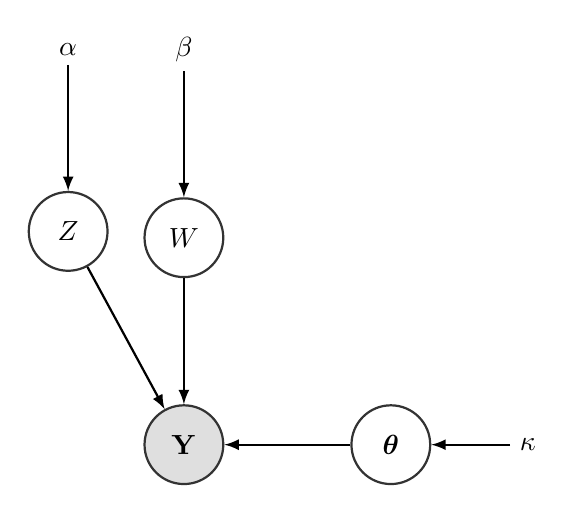
\begin{tikzpicture}
		\tikzstyle{main}=[circle, minimum size = 10mm, thick, draw =black!80, node distance = 16mm]
		\tikzstyle{connect}=[-latex, thick]
		%\tikzstyle{box}=[rectangle, draw=black!100]
		\node[ fill = white!100] (alpha) {$\alpha$};
		\node[main] (Z) [below=of alpha] {$Z$};
		
		\node[] (beta) [right=of alpha] {$\beta$};
		\node[main] (W) [below=of beta] {$W$};
		
		\node[main, fill = gray!25] (Y) [below=of W] {$\mathbf{Y}$};
		\node[main] (theta) [right=of Y] {$\boldsymbol{\theta}$};
		
		\node[] (kappa) [right=of theta] {$\kappa$};
		
		\path (Z) edge [connect] (Y);
		\path (W) edge [connect] (Y);
		
		\path (theta) edge [connect] (Y);
		
		\path (alpha) edge [connect] (Z);
		\path (beta) edge [connect] (W);
		
		\path (kappa) edge [connect] (theta);
		
		%\node[rectangle, inner sep=0mm, fit= (z) (w),label=below right:N, xshift=13mm] {};
		%\node[rectangle, inner sep=4.4mm,draw=black!100, fit= (z) (w)] {};
		%\node[rectangle, inner sep=4.6mm, fit= (z) (w),label=below right:M, xshift=12.5mm] {};
		%\node[rectangle, inner sep=9mm, draw=black!100, fit = (theta) (z) (w)] {};
	\end{tikzpicture}
\end{figure}	


\section{Estimation}

The likelihood of the model parameter $\boldsymbol{\tau}$ equals
$$
L(\boldsymbol{\theta}) = \sum_{(z, w) \in \mathcal{Z}, \mathcal{W}} \prod_{i, g} \alpha^{z_{ig}} \prod_{j, l} \beta^{w_{jl}} \prod_{i, j, g, l} \varphi(\mathbf{y}_{ij}; \theta_{gl})^{z_{ig} w_{jl}}
$$

So should we model $\varphi(\cdot)$ as a bivariate beta distribution (meaning Dirichlet distribution)? Regarding this, see the paper "Time Series of Continuous Proportions", by Grunwald, Raftery and Guttorp (1993), where they model the time series of proportions using the Dirichlet distribution.


There is a paper ("Estimation and selection for the latent block model on categorical data" by Keribin et al.) that implements the LBM for multinomial data that in the estimation of the model sets prior distributions for the mixing proportions as well as the parameter that governs the $Y$ distribution. This would in a sense be similar to our case, since the eSIR model imposes a Dirichlet prior on the $\boldsymbol{\theta}$ parameter. If we would further impose Dirichlet priors on the mixing proportions, would we be able to do something similar as in Keribin et al.?

So specifically, following \parencite{keribin2015estimation} we can consider proper and non-informative priors for $\alpha$ and $\beta$ as
%
\begin{equation}
	\begin{aligned}
		\boldsymbol{\alpha} \sim \text{Dirichlet}(a, \ldots, a) \\
		%
		\boldsymbol{\beta} \sim \text{Dirichlet}(a, \ldots, a)
	\end{aligned}
\end{equation}
%

In \parencite{keribin2015estimation} they consider a very similar general modeling structure and estimate the model parameters $\boldsymbol{\tau}$ by maximizing the posterior density $p(\boldsymbol{\tau} | \boldsymbol{y})$, which leads to the Maximum A Posteriori (MAP) estimator: 
%
\begin{equation}
	\hat{\boldsymbol{\tau}}_{MAP} = \underset{\boldsymbol{\tau}}{\mathrm{argmax}} \: p(\boldsymbol{\tau} | \boldsymbol{y})
\end{equation}
 
We would thus be able to graphically represent the model as 
%
\begin{figure}[H]
	\centering
	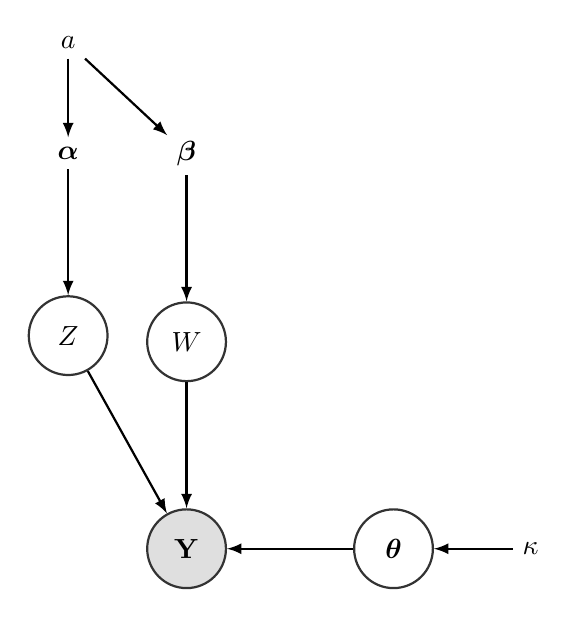
\begin{tikzpicture}
		\tikzstyle{main}=[circle, minimum size = 10mm, thick, draw =black!80, node distance = 16mm]
		\tikzstyle{connect}=[-latex, thick]
		%\tikzstyle{box}=[rectangle, draw=black!100]
		\node[ fill = white!100] (alpha) {$\boldsymbol{\alpha}$};
		\node[main] (Z) [below=of alpha] {$Z$};
		
		\node[] (a) [above= of alpha] {$a$}; 
		
		\node[] (beta) [right=of alpha] {$\boldsymbol{\beta}$};
		\node[main] (W) [below=of beta] {$W$};
		
		\node[main, fill = gray!25] (Y) [below=of W] {$\mathbf{Y}$};
		\node[main] (theta) [right=of Y] {$\boldsymbol{\theta}$};
		
		\node[] (kappa) [right=of theta] {$\kappa$};
		
		\path (Z) edge [connect] (Y);
		\path (W) edge [connect] (Y);
		
		\path (a) edge [connect] (alpha);
		\path (a) edge [connect] (beta);
		
		\path (theta) edge [connect] (Y);
		
		\path (alpha) edge [connect] (Z);
		\path (beta) edge [connect] (W);
		
		\path (kappa) edge [connect] (theta);

	\end{tikzpicture}
\end{figure}



\printbibliography

\end{document}